\documentclass[aspectratio=169]{beamer}
\usetheme{oxfordmaths}

\usepackage{caption}
\usepackage{subcaption}

\title[Differentiable Electrochemical Simulation]
{Differentiable Electrochemical Simulation for Gradient-Based
Parameter Inference}
\author{Jack Montgomery}
\institute{Mathematical Institute\\University of Oxford}
\date[March 2025]
{OMMS Dissertation Presentation}

\begin{document}

\begin{frame}[plain]
  \titlepage
\end{frame}

\begin{frame}
  \frametitle{Electrochemistry and Cyclic Voltammetry}
  \begin{figure}[h!]
    \centering
    \begin{subfigure}[b]{0.45\textwidth}
      \centering
      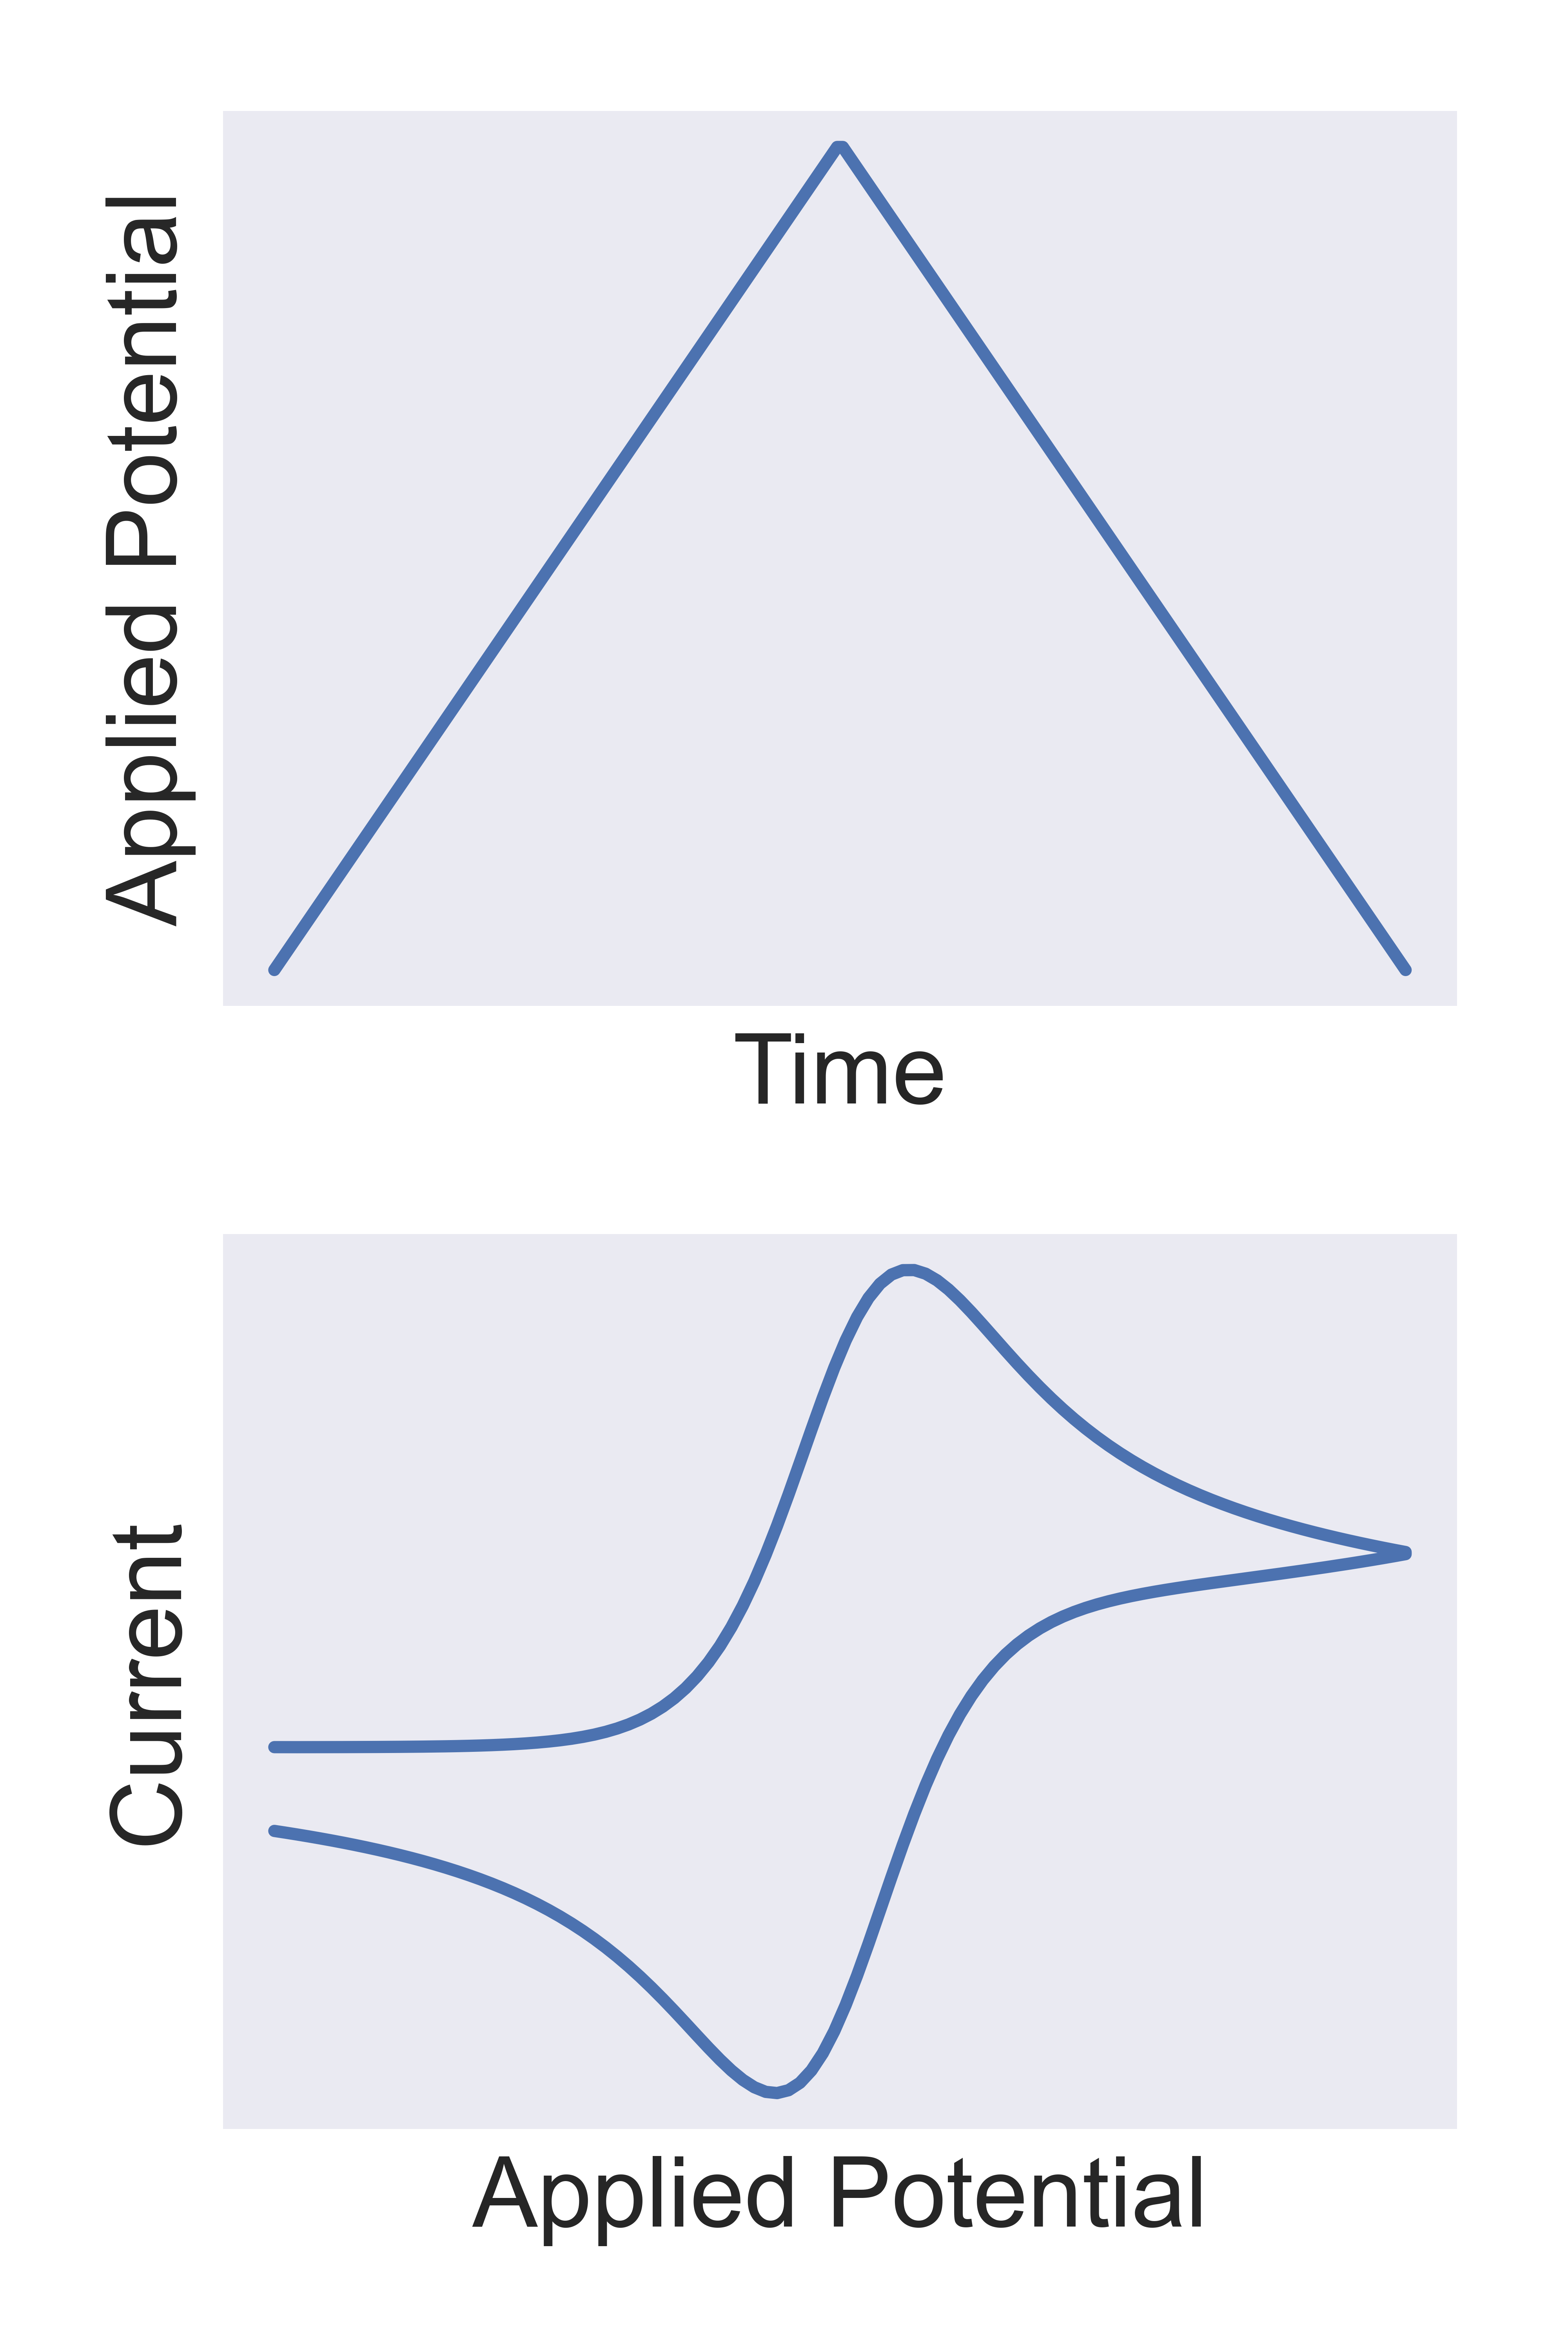
\includegraphics[width=\textwidth]{figures/cyclic-voltammetry.png}
    \end{subfigure}
    \pause
    \hfill
    \begin{subfigure}[b]{0.45\textwidth}
      \centering
      \includegraphics[scale=0.4]{figures/voltammagram.png}
    \end{subfigure}
  \end{figure}
\end{frame}

\begin{frame}
  \frametitle{Mathematical Description}
  \begin{itemize}
    \item \textbf{Diffusion}:
      \begin{itemize}
        \item $\frac{\partial c_A}{\partial t} = D_A
          \frac{\partial^2 c_A}{\partial x^2}$
        \item $\frac{\partial c_B}{\partial t} = D_A
          \frac{\partial^2 c_B}{\partial x^2}$
      \end{itemize}

    \item \textbf{Initial Condition}: $c_A(0, x) = c_A^*, \ c_B(0, x) = c_B^*$
    \item \textbf{Infinite Boundary Conditions}:
      \begin{itemize}
        \item $c_A(t, x) \to c_A^* \text{ as } x \to \infty$
        \item $c_B(t, x) \to c_B^* \text{ as } x \to \infty$
      \end{itemize}
    \item \textbf{Electrode Boundary Condition} (Butler-Volmer):
      \begin{itemize}
        \item $D_A \frac{\partial c_A}{\partial x}\bigg|_{x=0} =
          k_0 \left[ c_A(t,0)\, e^{-\alpha \frac{F}{RT} (E(t) - E^0_f)}
          - c_B(t,0)\, e^{(1-\alpha) \frac{F}{RT} (E(t) - E^0_f)} \right]$
        \item $D_B \frac{\partial c_B}{\partial x}\bigg|_{x=0} = - D_A
          \frac{\partial c_A}{\partial x}\bigg|_{x=0}$
      \end{itemize}
    \item \textbf{Current:} $I = F A j_{0, A}$ where $ j_{0, A} = - D
      \frac{\partial c_A}{\partial x}\bigg|_{x=0}$
  \end{itemize}
\end{frame}

\begin{frame}
  \frametitle{Mathematical Description}
  Assuming $D_A = D_B$
  \begin{itemize}
    \item \textbf{Diffusion}: $\frac{\partial C_A}{\partial t} =
      \frac{\partial^2 C_A}{\partial x^2}$
    \item \textbf{Initial Condition}: $C_A(0, X) = 1$
    \item \textbf{Infinite Boundary Conditions}: $C_A(t, X_{\text{max}}) = 1$
    \item \textbf{Electrode Boundary Condition} (Butler-Volmer):
      $\frac{\partial C_A}{\partial X}\bigg|_{X=0} =
      K_0 \left[ C_A(T,0)\, e^{-\alpha (\theta(T) - \theta^0_f)}
      - (1 - C_A(T,0))\, e^{(1-\alpha) (\theta(T) - \theta^0_f)} \right]$
    \item \textbf{Current:} $I = \pi \epsilon F D_A  c^*_A J_{0, A}$
      where $ J_{0, A} = - D
      \frac{\partial C_A}{\partial X}\bigg|_{X=0}$
  \end{itemize}
\end{frame}

\begin{frame}
  \frametitle{Forward Problem}
  \begin{itemize}
    \item Set $\phi = \left( \alpha, K_0, \theta_f \right)$
    \item Finite Difference Solver: $\mathcal{P}(\phi) = J$
  \end{itemize}
  % NOTE: I need to change the heading in the plots
  
\includegraphics[scale=0.45]{figures/forward-problem.png}
\end{frame}

\begin{frame}
  \frametitle{Inverse Problem}
  \begin{center}
    \begin{minipage}[c]{0.5\textwidth}
      \centering
      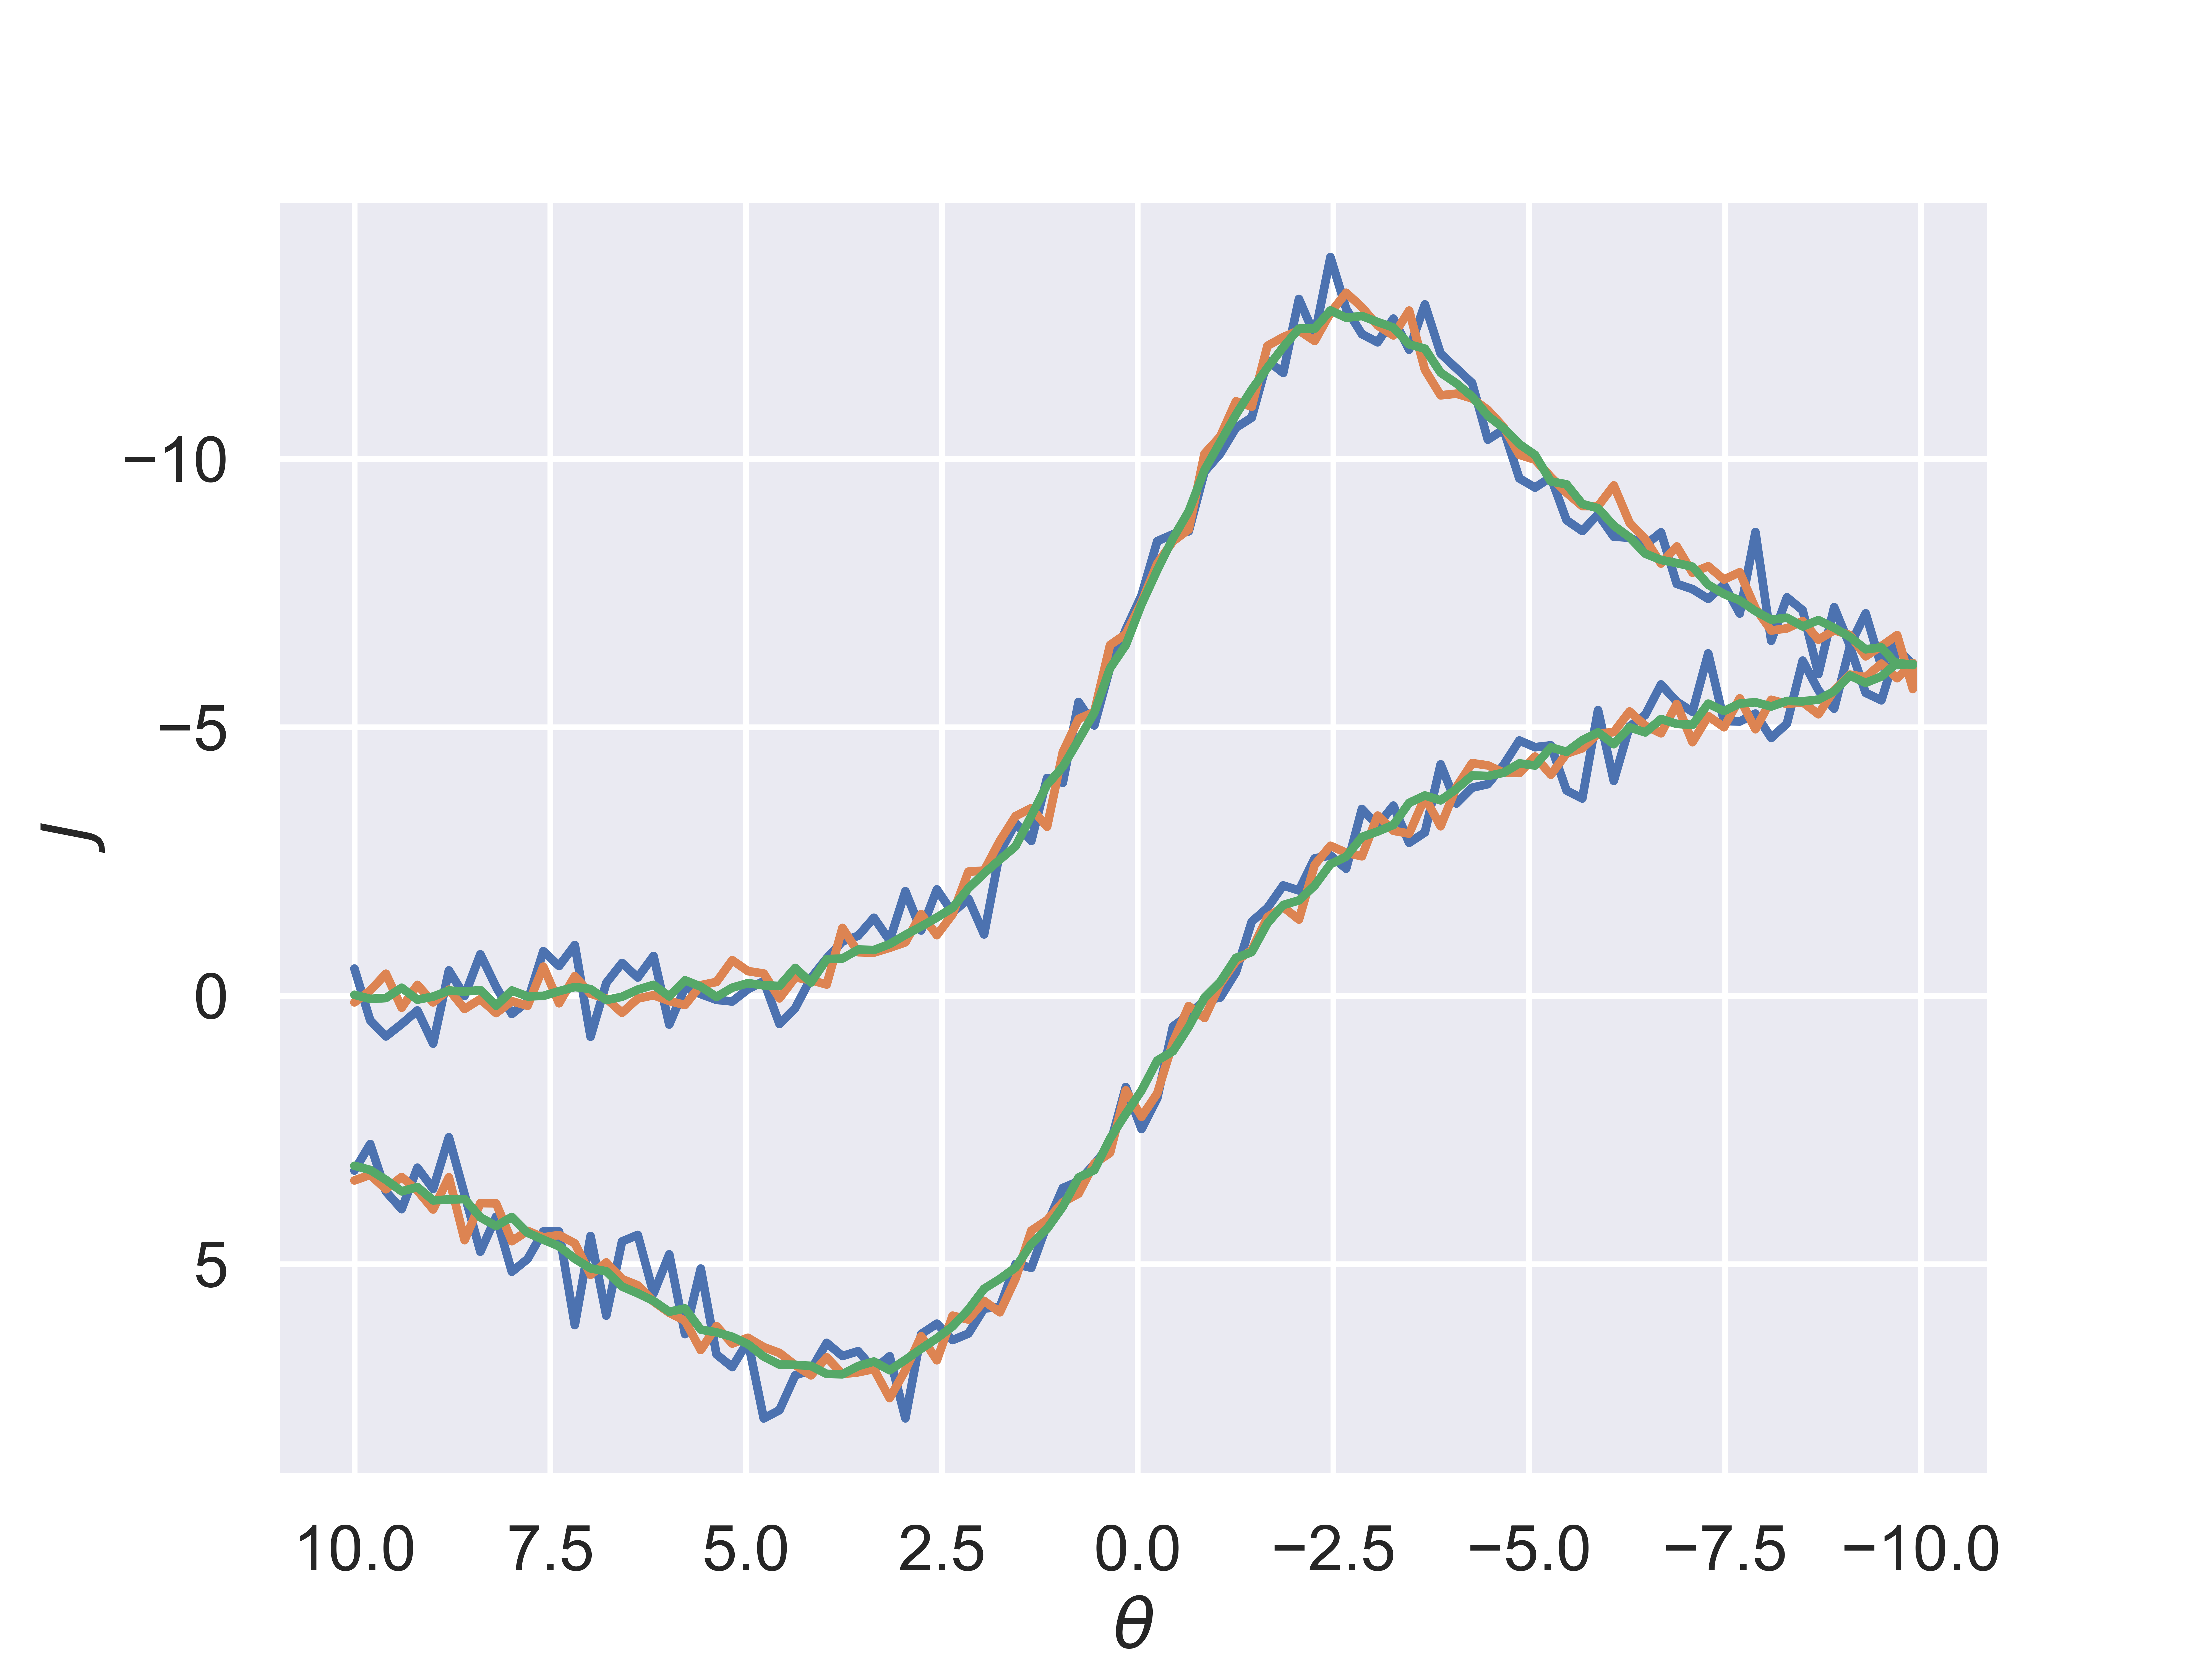
\includegraphics[scale=0.3]{figures/noisy-samples.png}
    \end{minipage}
    \hspace{0.3cm}
    $\longrightarrow$
    \hspace{0.3cm}
    \begin{minipage}[c]{0.2\textwidth}
      \centering
      $\phi$
    \end{minipage}
  \end{center}
\end{frame}

%TODO: A slide on putting this into a Bayesian framing

\begin{frame}
  \frametitle{MCMC}
  \begin{itemize}
    \item Aim to approximate the posterior distribution $P(\phi |
      y)$, where $y$ is the experimental data
    \item Based on simulating a Markov chain whose limiting
      distribution is the posterior distribution
    \item Parameters are proposed based on a proposal distribution
      $q(\phi_{\text{cand} | \phi})$
    \item Proposals are accepted with probability: $$ r  = min\left\{
      \frac{L(\phi_{\text{cand}} | y)}{L(\theta_i | y)}, 1 \right\}$$
  \end{itemize}
\end{frame}

\begin{frame}
  \frametitle{Random-Walk Metropolis Hastings}
  $q(\theta|\theta_t) \sim \mathcal{N}(0, \Sigma)$ %NOTE: This is not
  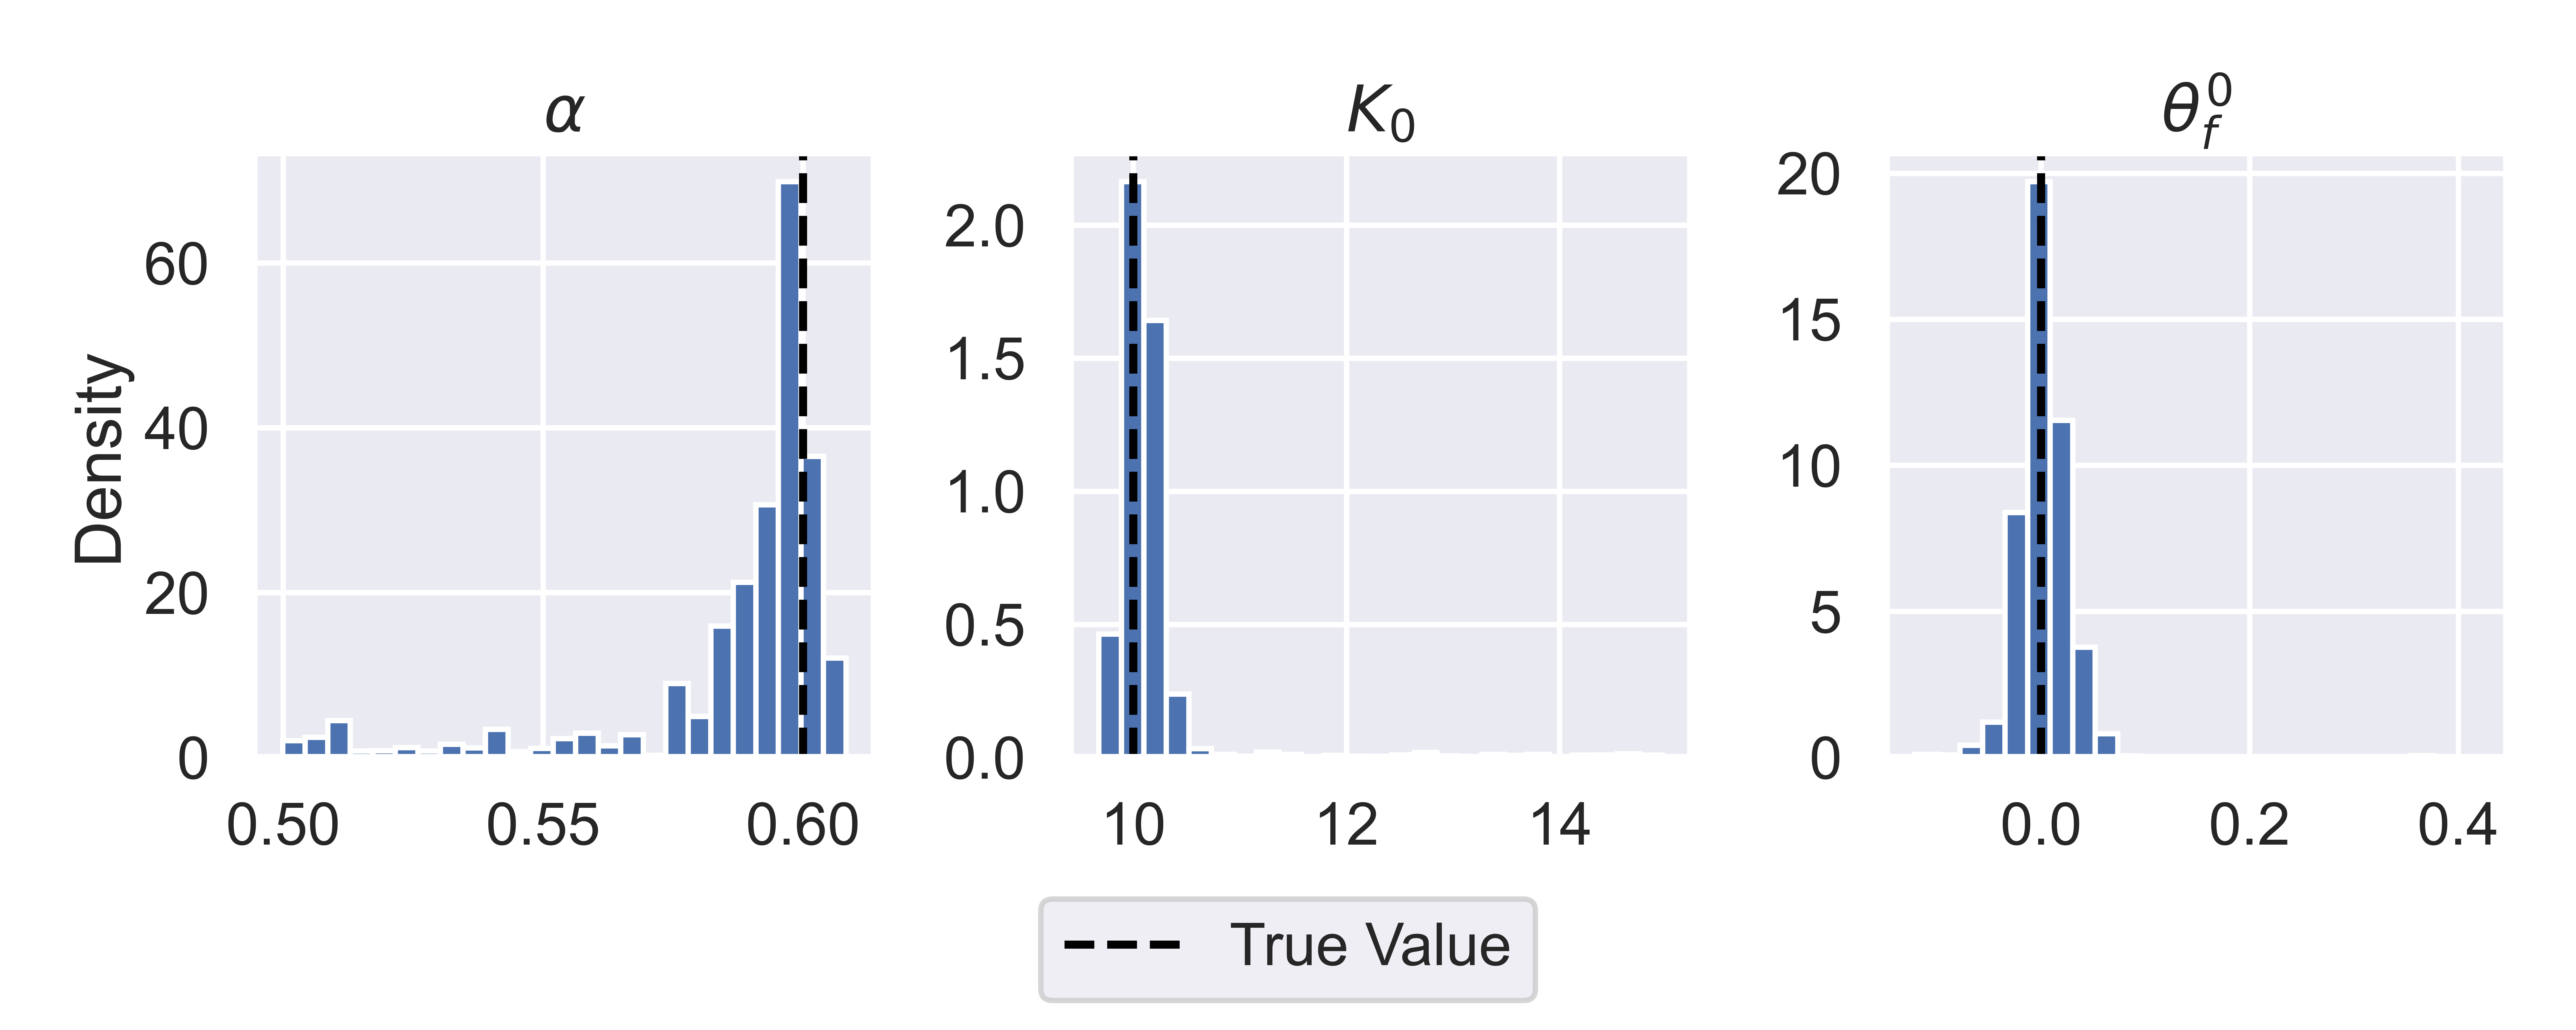
\includegraphics[scale=0.5]{figures/no-burn-in.png}
\end{frame}

\begin{frame}
  \frametitle{Burn-in}
  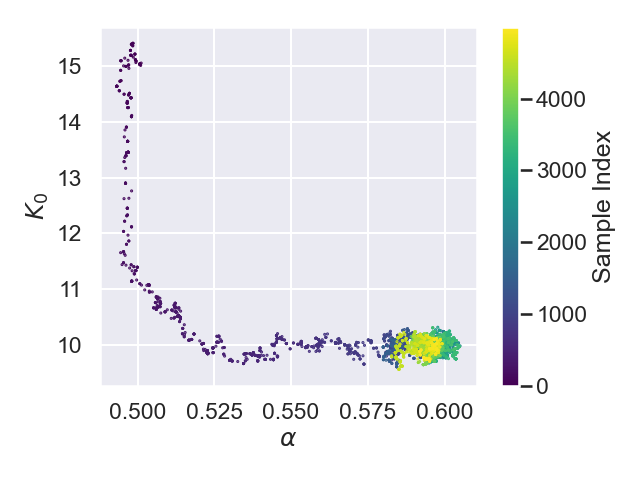
\includegraphics[scale=0.5]{figures/normal-burn-in.png}
\end{frame}

\begin{frame}
  \frametitle{Differentiable Simulator}
  \begin{itemize}
    \item $\mathcal{P}$ is a composition of differentiable functions
      so it is itself differentiable.
    \item Hard to derive analytically, but we can compute the
      dervatives efficiently using automatic differentiation
    \item Compute $\Delta_{\phi} L$
  \end{itemize}
\end{frame}

\begin{frame}
  \frametitle{Burn-in}
  Performing gradient descent on the
  likelihood can help us enter areas of high density faster.
  \includegraphics[scale=0.35]{figures/burn-in-comparison.png}
  % TODO: Plot of the gradient descent steps for K_0 and \alpha
  % TODO: Plot of the posterior
\end{frame}

\begin{frame}
  \frametitle{Hamiltonian Monte Carlo}
\end{frame}

\begin{frame}
  \frametitle{Further Work}
\end{frame}

\end{document}
